\documentclass[11pt,twoside]{article}

\usepackage[table,xcdraw]{xcolor}
\usepackage{float}

\newcommand{\reporttitle}{Introduction to Machine Learning}

\newcommand{\reporttype}{Coursework 2 \\ \vspace{0.5cm} Neural Networks}
\newcommand{\probdef}[1]{\textbf{Problem:}  #1 \\ \\ \textbf{Answer:}}

% include files that load packages and define macros
%%%%%%%%%%%%%%%%%%%%%%%%%%%%%%%%%%%%%%%%%
% University Assignment Title Page 
% LaTeX Template
% Version 1.0 (27/12/12)
%
% This template has been downloaded from:
% http://www.LaTeXTemplates.com
%
% Original author:
% WikiBooks (http://en.wikibooks.org/wiki/LaTeX/Title_Creation)
%
% License:
% CC BY-NC-SA 3.0 (http://creativecommons.org/licenses/by-nc-sa/3.0/)
% 
% Instructions for using this template:
% This title page is capable of being compiled as is. This is not useful for 
% including it in another document. To do this, you have two options: 
%
% 1) Copy/paste everything between \begin{document} and \end{document} 
% starting at \begin{titlepage} and paste this into another LaTeX file where you 
% want your title page.
% OR
% 2) Remove everything outside the \begin{titlepage} and \end{titlepage} and 
% move this file to the same directory as the LaTeX file you wish to add it to. 
% Then add \input{./title_page_1.tex} to your LaTeX file where you want your
% title page.
%
%----------------------------------------------------------------------------------------
%	PACKAGES AND OTHER DOCUMENT CONFIGURATIONS
%----------------------------------------------------------------------------------------
\usepackage{ifxetex}
\usepackage{textpos}
\usepackage{natbib}
\usepackage{kpfonts}
\usepackage[a4paper,hmargin=2.8cm,vmargin=2.0cm,includeheadfoot]{geometry}
\usepackage{ifxetex}
\usepackage{stackengine}
\usepackage{tabularx,longtable,multirow,subfigure,caption}%hangcaption
\usepackage{fncylab} %formatting of labels
\usepackage{fancyhdr}
\usepackage{color}
\usepackage[tight,ugly]{units}
\usepackage{url}
\usepackage{float}
\usepackage[english]{babel}
\usepackage{amsmath}
\usepackage{graphicx}
\usepackage[colorinlistoftodos]{todonotes}
\usepackage{dsfont}
\usepackage{epstopdf} % automatically replace .eps with .pdf in graphics
\usepackage{natbib}
\usepackage{backref}
\usepackage{array}
\usepackage{latexsym}
\usepackage{etoolbox}

\usepackage{enumerate} % for numbering with [a)] format 



\ifxetex
\usepackage{fontspec}
\setmainfont[Scale=.8]{OpenDyslexic-Regular}
\else
\usepackage[pdftex,pagebackref,hypertexnames=false,colorlinks]{hyperref} % provide links in pdf
\hypersetup{pdftitle={},
  pdfsubject={}, 
  pdfauthor={\reportauthor},
  pdfkeywords={}, 
  pdfstartview=FitH,
  pdfpagemode={UseOutlines},% None, FullScreen, UseOutlines
  bookmarksnumbered=true, bookmarksopen=true, colorlinks,
    citecolor=black,%
    filecolor=black,%
    linkcolor=black,%
    urlcolor=black}
\usepackage[all]{hypcap}
\fi

\usepackage{tcolorbox}

% various theorems
\usepackage{ntheorem}
\theoremstyle{break}
\newtheorem{lemma}{Lemma}
\newtheorem{theorem}{Theorem}
\newtheorem{remark}{Remark}
\newtheorem{definition}{Definition}
\newtheorem{proof}{Proof}

% example-environment
\newenvironment{example}[1][]
{ 
\vspace{4mm}
\noindent\makebox[\linewidth]{\rule{\hsize}{1.5pt}}
\textbf{Example #1}\\
}
{ 
\noindent\newline\makebox[\linewidth]{\rule{\hsize}{1.0pt}}
}



%\renewcommand{\rmdefault}{pplx} % Palatino
% \renewcommand{\rmdefault}{put} % Utopia

\ifxetex
\else
\renewcommand*{\rmdefault}{bch} % Charter
\renewcommand*{\ttdefault}{cmtt} % Computer Modern Typewriter
%\renewcommand*{\rmdefault}{phv} % Helvetica
%\renewcommand*{\rmdefault}{iwona} % Avant Garde
\fi

\setlength{\parindent}{0em}  % indentation of paragraph

\setlength{\headheight}{14.5pt}
\pagestyle{fancy}
\fancyfoot[ER,OL]{\thepage}%Page no. in the left on
                                %odd pages and on right on even pages
\fancyfoot[OC,EC]{\sffamily }
\renewcommand{\headrulewidth}{0.1pt}
\renewcommand{\footrulewidth}{0.1pt}
\captionsetup{margin=10pt,font=small,labelfont=bf}


%--- chapter heading

\def\@makechapterhead#1{%
  \vspace*{10\p@}%
  {\parindent \z@ \raggedright %\sffamily
        %{\Large \MakeUppercase{\@chapapp} \space \thechapter}
        %\\
        %\hrulefill
        %\par\nobreak
        %\vskip 10\p@
    \interlinepenalty\@M
    \Huge \bfseries 
    \thechapter \space\space #1\par\nobreak
    \vskip 30\p@
  }}

%---chapter heading for \chapter*  
\def\@makeschapterhead#1{%
  \vspace*{10\p@}%
  {\parindent \z@ \raggedright
    \sffamily
    \interlinepenalty\@M
    \Huge \bfseries  
    #1\par\nobreak
    \vskip 30\p@
  }}
  



% %%%%%%%%%%%%% boxit
\def\Beginboxit
   {\par
    \vbox\bgroup
	   \hrule
	   \hbox\bgroup
		  \vrule \kern1.2pt %
		  \vbox\bgroup\kern1.2pt
   }

\def\Endboxit{%
			      \kern1.2pt
		       \egroup
		  \kern1.2pt\vrule
		\egroup
	   \hrule
	 \egroup
   }	

\newenvironment{boxit}{\Beginboxit}{\Endboxit}
\newenvironment{boxit*}{\Beginboxit\hbox to\hsize{}}{\Endboxit}



\allowdisplaybreaks

\makeatletter
\newcounter{elimination@steps}
\newcolumntype{R}[1]{>{\raggedleft\arraybackslash$}p{#1}<{$}}
\def\elimination@num@rights{}
\def\elimination@num@variables{}
\def\elimination@col@width{}
\newenvironment{elimination}[4][0]
{
    \setcounter{elimination@steps}{0}
    \def\elimination@num@rights{#1}
    \def\elimination@num@variables{#2}
    \def\elimination@col@width{#3}
    \renewcommand{\arraystretch}{#4}
    \start@align\@ne\st@rredtrue\m@ne
}
{
    \endalign
    \ignorespacesafterend
}
\newcommand{\eliminationstep}[2]
{
    \ifnum\value{elimination@steps}>0\leadsto\quad\fi
    \left[
        \ifnum\elimination@num@rights>0
            \begin{array}
            {@{}*{\elimination@num@variables}{R{\elimination@col@width}}
            |@{}*{\elimination@num@rights}{R{\elimination@col@width}}}
        \else
            \begin{array}
            {@{}*{\elimination@num@variables}{R{\elimination@col@width}}}
        \fi
            #1
        \end{array}
    \right]
    & 
    \begin{array}{l}
        #2
    \end{array}
    &%                                    moved second & here
    \addtocounter{elimination@steps}{1}
}
\makeatother

%% Fast macro for column vectors
\makeatletter  
\def\colvec#1{\expandafter\colvec@i#1,,,,,,,,,\@nil}
\def\colvec@i#1,#2,#3,#4,#5,#6,#7,#8,#9\@nil{% 
  \ifx$#2$ \begin{bmatrix}#1\end{bmatrix} \else
    \ifx$#3$ \begin{bmatrix}#1\\#2\end{bmatrix} \else
      \ifx$#4$ \begin{bmatrix}#1\\#2\\#3\end{bmatrix}\else
        \ifx$#5$ \begin{bmatrix}#1\\#2\\#3\\#4\end{bmatrix}\else
          \ifx$#6$ \begin{bmatrix}#1\\#2\\#3\\#4\\#5\end{bmatrix}\else
            \ifx$#7$ \begin{bmatrix}#1\\#2\\#3\\#4\\#5\\#6\end{bmatrix}\else
              \ifx$#8$ \begin{bmatrix}#1\\#2\\#3\\#4\\#5\\#6\\#7\end{bmatrix}\else
                 \PackageError{Column Vector}{The vector you tried to write is too big, use bmatrix instead}{Try using the bmatrix environment}
              \fi
            \fi
          \fi
        \fi
      \fi
    \fi
  \fi 
}  
\makeatother

\robustify{\colvec}

%%% Local Variables: 
%%% mode: latex
%%% TeX-master: "notes"
%%% End: 
 % various packages needed for maths etc.
% quick way of adding a figure
\newcommand{\fig}[3]{
 \begin{center}
 \scalebox{#3}{\includegraphics[#2]{#1}}
 \end{center}
}

%\newcommand*{\point}[1]{\vec{\mkern0mu#1}}
\newcommand{\ci}[0]{\perp\!\!\!\!\!\perp} % conditional independence
\newcommand{\point}[1]{{#1}} % points 
\renewcommand{\vec}[1]{{\boldsymbol{{#1}}}} % vector
\newcommand{\mat}[1]{{\boldsymbol{{#1}}}} % matrix
\newcommand{\R}[0]{\mathds{R}} % real numbers
\newcommand{\Z}[0]{\mathds{Z}} % integers
\newcommand{\N}[0]{\mathds{N}} % natural numbers
\newcommand{\nat}[0]{\mathds{N}} % natural numbers
\newcommand{\Q}[0]{\mathds{Q}} % rational numbers
\ifxetex
\newcommand{\C}[0]{\mathds{C}} % complex numbers
\else
\newcommand{\C}[0]{\mathds{C}} % complex numbers
\fi
\newcommand{\tr}[0]{\text{tr}} % trace
\renewcommand{\d}[0]{\mathrm{d}} % total derivative
\newcommand{\inv}{^{-1}} % inverse
\newcommand{\id}{\mathrm{id}} % identity mapping
\renewcommand{\dim}{\mathrm{dim}} % dimension
\newcommand{\rank}[0]{\mathrm{rk}} % rank
\newcommand{\determ}[1]{\mathrm{det}(#1)} % determinant
\newcommand{\scp}[2]{\langle #1 , #2 \rangle}
\newcommand{\kernel}[0]{\mathrm{ker}} % kernel/nullspace
\newcommand{\img}[0]{\mathrm{Im}} % image
\newcommand{\idx}[1]{{(#1)}}
\DeclareMathOperator*{\diag}{diag}
\newcommand{\E}{\mathds{E}} % expectation
\newcommand{\var}{\mathds{V}} % variance
\newcommand{\gauss}[2]{\mathcal{N}\big(#1,\,#2\big)} % gaussian distribution N(.,.)
\newcommand{\gaussx}[3]{\mathcal{N}\big(#1\,|\,#2,\,#3\big)} % gaussian distribution N(.|.,.)
\newcommand{\gaussBig}[2]{\mathcal{N}\left(#1,\,#2\right)} % see above, but with brackets that adjust to the height of the arguments
\newcommand{\gaussxBig}[3]{\mathcal{N}\left(#1\,|\,#2,\,#3\right)} % see above, but with brackets that adjust to the height of the arguments
\DeclareMathOperator{\cov}{Cov} % covariance (matrix) 
\ifxetex
\renewcommand{\T}[0]{^\top} % transpose
\else
\newcommand{\T}[0]{^\top}
\fi
% matrix determinant
\newcommand{\matdet}[1]{
\left|
\begin{matrix}
#1
\end{matrix}
\right|
}



%%% various color definitions
\definecolor{darkgreen}{rgb}{0,0.6,0}

\newcommand{\blue}[1]{{\color{blue}#1}}
\newcommand{\red}[1]{{\color{red}#1}}
\newcommand{\green}[1]{{\color{darkgreen}#1}}
\newcommand{\orange}[1]{{\color{orange}#1}}
\newcommand{\magenta}[1]{{\color{magenta}#1}}
\newcommand{\cyan}[1]{{\color{cyan}#1}}


% redefine emph
\renewcommand{\emph}[1]{\blue{\bf{#1}}}

% place a colored box around a character
\gdef\colchar#1#2{%
  \tikz[baseline]{%
  \node[anchor=base,inner sep=2pt,outer sep=0pt,fill = #2!20] {#1};
    }%
}%
 % short-hand notation and macros

%%%%%%%%%%%%%%%%%%%%%%%%%%%%
\setlength{\parindent}{1cm} % Default is 15pt.

\begin{document}
% front page
% Last modification: 2016-09-29 (Marc Deisenroth)
\begin{titlepage}

\newcommand{\HRule}{\rule{\linewidth}{0.5mm}} % Defines a new command for the horizontal lines, change thickness here


%----------------------------------------------------------------------------------------
%	LOGO SECTION
%----------------------------------------------------------------------------------------


\includegraphics[width = 4cm]{./figures/imperial}\\[0.5cm] 

\begin{center} % Center remainder of the page

%----------------------------------------------------------------------------------------
%	HEADING SECTIONS
%----------------------------------------------------------------------------------------
\textsc{\LARGE \reporttype}\\[1.5cm] 
\textsc{\Large Imperial College London}\\[0.5cm] 
\textsc{\large Department of Computing}\\[0.5cm] 
%----------------------------------------------------------------------------------------
%	TITLE SECTION
%----------------------------------------------------------------------------------------

\HRule \\[0.4cm]
{ \huge \bfseries \reporttitle}\\ % Title of your document
\HRule \\[1.5cm]
\end{center}
%----------------------------------------------------------------------------------------
%	AUTHOR SECTION
%----------------------------------------------------------------------------------------

%\begin{minipage}{0.4\hsize}
\begin{flushleft} \large
\textit{Author:}\\
\reportauthor~(CID: \cid) \\% Your name 
\textit{Email:} \\
\reportemail
\end{flushleft}
\vspace{2cm}
\makeatletter
Date: \@date 

\vfill % Fill the rest of the page with whitespace



\makeatother


\end{titlepage}



\thispagestyle{empty}
\renewcommand{\contentsname}{Table of Contents}
\setcounter{tocdepth}{2}
{\hypersetup{linkcolor=black} % Locally black links so they don't stand out here
\tableofcontents
% \addtocontents{toc}{\par\nobreak \mbox{}\hfill{\bf Page}\par\nobreak}
% \newpage
%

% \addtocontents{lot}{\par\nobreak\textbf{{\scshape Table} \hfill Page}\par\nobreak}
%
\listoffigures
% \addtocontents{lof}{\par\nobreak\textbf{{\scshape Figure} \hfill Page}\par\nobreak}
\listoftables

}
\newpage
%%%%%%%%%%%%%%%%%%%%%%%%%%%% Main document

\setcounter{page}{1}
\section{Overview}

We present our implementations of claim classifiers built using Keras and Tensorflow \cite{chollet2015keras,tensorflow} for the purpose of pricing automotive insurance, with training performed on a historical insurance dataset. In Part 2, we create a binary classifier to predict whether a client is likely to make a claim, and tune the classifier's model after addressing the imbalanced nature of the dataset. In Part 3 we develop a pricing model based on the claim prediction model from Part 2 coupled with a tuned severity model. This model is then tested and tuned based on its performance in a competitive insurance market populated with competing AI insurance policy offerers. 
\section{Insurance Claim Classification}

\subsection{Implementation}

\subsubsection*{Data Exploration} \label{section:explor}
\autoref{fig:corrplot} shows the correlation matrix for the \texttt{part2\_data.csv} (based on \cite{corr_plot}), in which variable pairs with strong positive correlations are shown in dark red and pairs with strong negative correlations shown in dark blue. This figure highlights that there are few strong correlations between the features, as illustrated by the weakness of colour for the first two columns in the figure. This in turn means that even a sophisticated model will struggle to accurately predict both class labels based on the features provided. 

Futhermore, \autoref{fig:pca} shows a representation of the dataset after undertaking dimensionality reduction using principal component analysis (PCA) with $n=2$ . Here we see that projecting the data in the two leading principal components (those with the greatest variance, i.e. most information about the data) results in largely overlapping distributions. From this we can deduce that the predictive power of the features in lieu of their labels, beyond the linear combination given by the PCA basis transformation, is subtle at best. In addition, we ran ordinary least squares regression on the dataset to further gauge the explanatory power of the features. Consistent with our findings from the PCA, very few variables provided statistically significant contributions. Consequently, we should expect linear models to perform relatively well on the dataset, and that adding additional complexity in the form of neural networks is likely to yield only marginal improvements which themselves will require the successful identification of necessarily sub-leading non-linear relationships in the data (these ideas are developed further in \autoref{sec:linmodel}).

Indeed, while trialling our initial neural network models on the dataset we found three features, \texttt{vh\_cyl, vh\_din, vh\_sale\_begin}, with negligible explanatory power, and consequently chose to omit these from the input data. The remaining variables chosen to be included in the binary classification task were \texttt{drv\_age1} (driver's age), \texttt{vh\_age} (vehicle's age), \texttt{pol\_bonus} (bonus coefficient), \texttt{vh\_sale\_end} (years for which the vehicle has been out of production), \texttt{vh\_value} (vehicle's value), \texttt{vh\_speed} (vehicle's maximum speed). 

\subsubsection*{Data Preprocessing}
Normalization is performed by centering the distribution of every feature, and rescaling these to have unit variance. For this purpose, scikit-learn's \texttt{StandardScaler} was used \cite{scikit}. The corresponding transformation of a feature vector from the initial dataset $\vec{X}$ to the normalized dataset $\vec{z}$ is given by
\begin{equation}
\vec{z} = \frac{\vec{X}-m}{s},
\end{equation}
\noindent where $m=\frac{1}{n}\sum_{i=1}^{n}x_{i}$ is the sample mean and $s^2=\frac{1}{n} \sum_{i=1}^{n}{(x_{k}-m)}^2$ is the sample variance. Feature normalization is important for effectively training neural networks as, by removing the scale dependence of initial weights, it can make training faster as well as reducing the likelihood of getting stuck in local optima. Additionally, we ensure that feature normalization is carried out after splitting the dataset (for training and testing) to avoid "training" our scaler on the testing data; as such, the means and variances computed for the training data are used to rescale the test data \footnote{When other scalers were used the same ordering of procedures was respected, however, the relevant "learned" parameters were not necessarily the same.}.

It is worth noting that the provided insurance dataset is significantly unbalanced, with examples of contracts on which claims were made being underrepresented by 9:1. This imbalance needed to be addressed as neural network classifiers typically overfit on the over-represented class when trained on imbalanced data. One reason for this follows from the binary cross-entropy for data with labels $y$ and predicted labels $\^y$ which was used a loss function. From the functional form, 
\begin{equation}
-\sum_{i}^{N}y^{(i)}\log(\^{y}^{(i)})+(1-y^{(i)})\log(1-\^{y}^{(i)}),
\end{equation}

\noindent we see that the error from the majority class contributes significantly more toward the loss value than the minority class. As a result, this loss function is biased towards the majority class and fails to adequately capture the prediction errors over all classes.

In order to obtain a balanced dataset for training, naive random oversampling and undersampling methods were initially implemented, but more sophisticated methods presented in \cite{smote-comparison} were found to offer superior performance. In particular, we utilised the Synthetic Minority Oversampling Technique (SMOTE) \cite{Smote}, which oversamples the minority class by randomly picking a point from the minority class and computing the k-nearest neighbors for this point, and interpolating between these. Additionally, we also implemented a variant of SMOTE which utilizes Tomek Links \cite{smotetomek}. These essentially function to ensure that the nearest neighbors used for interpolation are only of the same class, thus theoretically providing more legitimate data (than vanilla SMOTE) for the classifier to train on. 

In order to ensure that the scaler is trained on purer data, and to reduce the effect of outliers (i.e. large variations in respective feature dimensions), we perform feature normalization before utilizing these oversampling techniques.

\subsubsection*{Neural Network Architecture}
\autoref{fig:part2model} shows the architecture of the network used for the binary classification task. Hidden layers were dense layers with ReLu activation functions, and the output layer was a single neuron with a sigmoid activation function, producing a single output between 0 and 1, interpretable as the confidence in predicting class 1\footnote{As we perform a cutoff at 0.5 for classification, the lack of probability calibration at this stage is not problematic.}. 
\begin{figure}[h!]
    \centering
    \makebox[\textwidth][c]{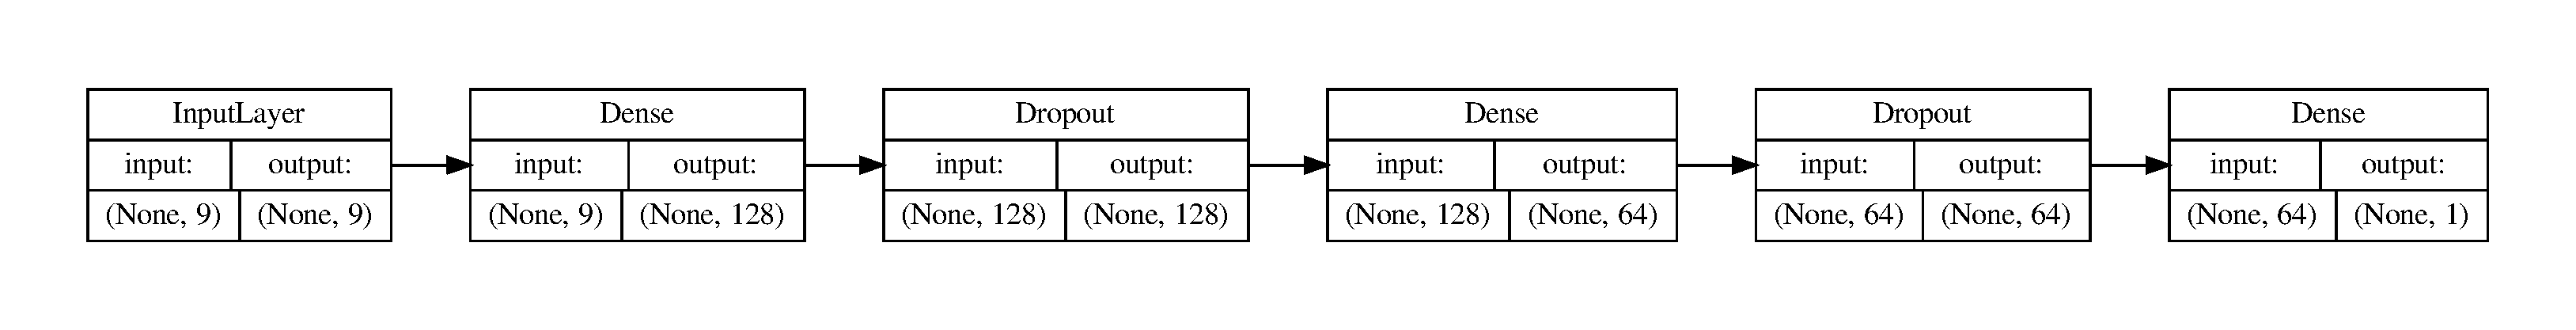
\includegraphics[width=1.2\textwidth]{figures/part2_model.pdf}}%
    \caption{Neural Network Architecture}
    \label{fig:part2model}
\end{figure}
\noindent
More details of the architecture and training parameters are given in \autoref{tab:part2initialnetworkparam}.

% Please add the following required packages to your document preamble:
% \usepackage[table,xcdraw]{xcolor}
% If you use beamer only pass "xcolor=table" option, i.e. \documentclass[xcolor=table]{beamer}
\begin{table}[]
\begin{tabular}{|l|l|l|l|l|l|}
\hline
\rowcolor[HTML]{EFEFEF} 
\textbf{Training Epochs} & \textbf{Batch Size} & \textbf{Activation Function} & \textbf{Dropout} & \textbf{Learning Rate} & \textbf{L2 Regularization} \\ \hline
10                  & 64                  & ReLu                         & 0                & 0.01                   & 0                          \\ \hline
\end{tabular}
\caption[Part 2: Initial Network Hyperparameters]{Initial Network Hyperparameters}
\label{tab:part2initialnetworkparam}
\end{table}
\noindent Owing to the complexity of the dataset, we used relatively large layer sizes in order to capture any interesting interactions between features and the target. The initial model did not significantly overfit the data, and achieved a relatively high (compared to more sophisticated models) AUC-ROC of 0.60. However, this was improved after doing a hyperparameter search which applied appropriate dropout and regularization values, which increased the AUC-ROC to 0.62. The purpose of regularization is to penalise large weights which has the effect of pushing weights toward zero, hence preventing overfitting and leading to more reliable learning.

\subsection{Architecture Evaluation}
\subsubsection*{Metrics}
The classification accuracy with an imbalanced dataset can be misleading. For instance, with the dataset analysed, a classifier predicting only the majority class will still have an classification accuracy of above 90\%.

To appropriately evaluate the performance, we first compute a confusion matrix where the columns represent predicted labels and rows represent ground truth labels. To account for the imbalances, we normalized the confusion matrix by row, i.e., by class, from which the recall and precision were derived.

 Recall is defined as 
\begin{equation}
\textnormal{Recall}=\frac{\textnormal{True Positive}}{\textnormal{True Positive}+\textnormal{False Negative}},
\end{equation}
capturing how well our model predicts the class compared to the true class of the instances. In particular, recall for the minority class was of particular interest to observe how well those who have made claims were being classified.

Precision is defined as
\begin{equation}
\textnormal{Precision}=\frac{\textnormal{True Positive}}{\textnormal{True Positive}+\textnormal{False Positive}},
\end{equation}
and provides a measure of how likely it is that an instance was from a particular class after the model predicted it was from that class. In particular, the precision for the majority class was of particular interest to observe how many of the minority class were being captured when predicted not to have made a claim.

In addition to the above, another key metric for evaluation was the AUC-ROC curve. The receiver operating characteristic (ROC) curve is a plot of the true positive rate against the false positive rate, defined as:
\begin{equation}
\textnormal{FPR}=\frac{\textnormal{False Positive}}{\textnormal{False Positive}+\textnormal{True Negative}},
\end{equation}
\noindent The true positive rate and false positive rate are traced out for every decision boundary, thereby the ROC curve is invariant to class ratios and the decision boundary. The area under the curve (AUC) is a measure of separability between the the classes and represents how well the model is able to distinguish between the the classes. A model with AUC equal to one is able to perfectly distinguish the classes whereas an AUC of 0.5 implies that the model is unable to separate the classes.

\subsubsection*{Initial Performance}

Due to the difficulty of classifying the provided dataset, as elucidated in Section 2.1.1, we strived to obtain a good initial architecture for the model that would be able to capture most of the inherent correlations between features and the target. The results we obtained were are provided in \autoref{tab:res1}.

% Please add the following required packages to your document preamble:
% \usepackage[table,xcdraw]{xcolor}
% If you use beamer only pass "xcolor=table" option, i.e. \documentclass[xcolor=table]{beamer}
\begin{table}[H]
\begin{tabular}{|
>{\columncolor[HTML]{EFEFEF}}l |lll|}
\hline
\textbf{}         & \multicolumn{1}{r|}{\cellcolor[HTML]{EFEFEF}\textbf{Normalized Precision}} & \multicolumn{1}{r|}{\cellcolor[HTML]{EFEFEF}\textbf{Normalized Recall}} & \cellcolor[HTML]{EFEFEF}\textbf{F1-Score} \\ \hline
\textbf{Class 0}  & \multicolumn{1}{r|}{0.59}                                                  & \multicolumn{1}{r|}{0.58}                                               & 0.58                                      \\ \hline
\textbf{Class 1}  & \multicolumn{1}{r|}{0.59}                                                  & \multicolumn{1}{r|}{0.60}                                               & 0.54                                      \\ \hline
\end{tabular}
\hfill
\begin{tabular}{|>{\columncolor[HTML]{EFEFEF}}l|r|}
\hline
\textbf{Accuracy} &  0.58 \\ \hline
\textbf{ROC-AUC}  &  0.60 \\ \hline
\end{tabular}
\caption[Part 2: Initial Network Performance]{Performance of the initial model}
\label{tab:res1}
\end{table}

\subsubsection*{Final Model Performance}

After hyperparameter tuning (see \autoref{sec:hyptune}), our final model had an AUC-ROC of 0.62, as shown in \autoref{tab:res2}.

\begin{table}[H]
\begin{tabular}{|
>{\columncolor[HTML]{EFEFEF}}l |lll|}
\hline
\textbf{}         & \multicolumn{1}{r|}{\cellcolor[HTML]{EFEFEF}\textbf{Normalized Precision}} & \multicolumn{1}{r|}{\cellcolor[HTML]{EFEFEF}\textbf{Normalized Recall}} & \cellcolor[HTML]{EFEFEF}\textbf{F1-Score} \\ \hline
\textbf{Class 0}  & \multicolumn{1}{r|}{0.60}                                                  & \multicolumn{1}{r|}{0.49}                                               & 0.58                                      \\ \hline
\textbf{Class 1}  & \multicolumn{1}{r|}{0.57}                                                  & \multicolumn{1}{r|}{0.67}                                               & 0.54                                      \\ \hline
\end{tabular}
\hfill
\begin{tabular}{|>{\columncolor[HTML]{EFEFEF}}l|r|}
\hline
\textbf{Accuracy} &  0.51 \\ \hline
\textbf{AUC-ROC}  &  0.62 \\ \hline
\end{tabular}
\caption[Part 2: Final Network Performance]{Performance of the final model}
\label{tab:res2}
\end{table}
\noindent
This is a marginal increase from the initial value of 0.60, but for difficult to classify real world data, this incremental increase can affect overall profits of the insurance company significantly. The difference in ROC curves can be seen in \autoref{fig:part2roc}. It is interesting to note that the accuracy went down after tuning, however, as mentioned previously, accuracy is not the best metric for evaluating model performance, and AUC-ROC serves as better estimate given the imbalanced nature of the data. \autoref{fig:part2roc} also shows us that optimizing the hyperparameters makes the graph more symmetrical, and increases the area under the curve, which is an indication of better model performance. 
\begin{figure}
    \centering
    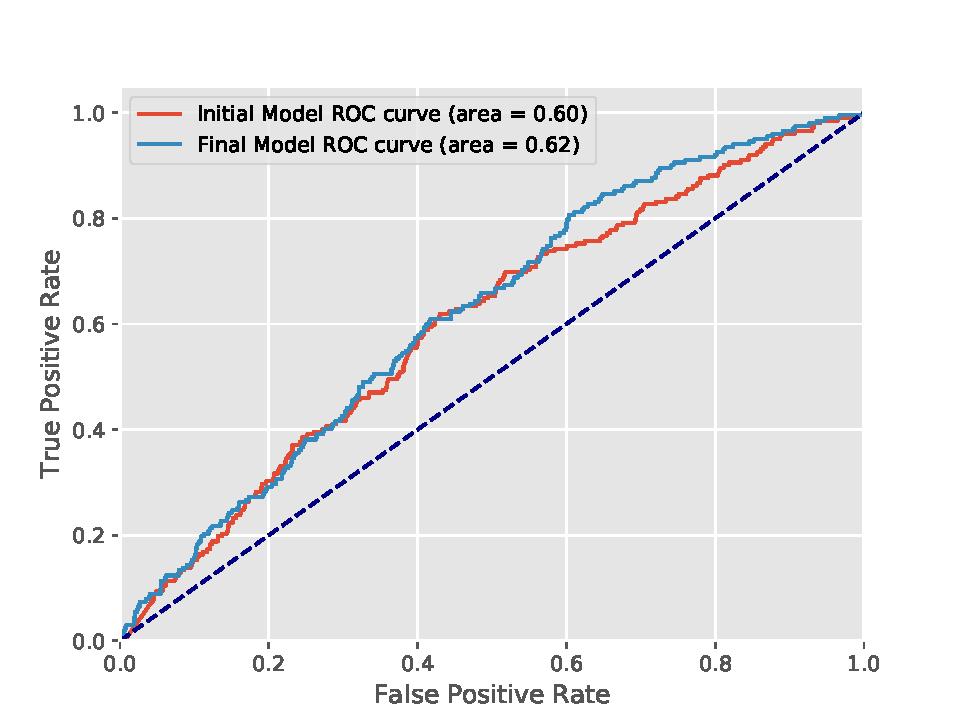
\includegraphics[width=0.7\textwidth]{figures/part2ROC.pdf}
    \caption[Part 2: ROC curves]{Part 2 ROC curves}
    \label{fig:part2roc}
\end{figure}

\subsection{Hyperparameter Tuning}
\label{sec:hyptune}
The key hyperparameters we were looking to optimise were the number of epochs, batch size, activation function, dropout rate, learning rate, and l2 regularization value. We optimised to the AUC-ROC as this provides a gauge of model performance which is independent of the decision boundary. The values used in the search are shown in \autoref{tab:hypparamsearch}.

% Please add the following required packages to your document preamble:
% \usepackage[table,xcdraw]{xcolor}
% If you use beamer only pass "xcolor=table" option, i.e. \documentclass[xcolor=table]{beamer}
\begin{table}[H]
\begin{tabular}{|l|l|l|l|l|l|}
\hline
\rowcolor[HTML]{EFEFEF} 
\textbf{Epoch Size} & \textbf{Batch Size} & \textbf{Activation Function} & \textbf{Dropout} & \textbf{Learning Rate} & \textbf{L2 Regularization} \\ \hline
5                   & 32                  & ReLu                         & 0                & 0.01                   & 0                          \\ \hline
10                  & 64                  & linear                       & 0.1              & 0.001                  & 0.01                       \\ \hline
20                  & 128                 &                              & 0.2              &                        & 0.001                      \\ \hline
                    &                     &                              & 0.3              &                        &                            \\ \hline
\end{tabular}
\caption{Configurations of hyperparameters used in the hyperparameter search.}
\label{tab:hypparamsearch}
\end{table}

The hyperparameter search was done over a search space comprising all combinations of the values shown in \autoref{tab:hypparamsearch}. This resulted in a search space of 432 distinct combinations. The search was done on all combinations at once as optimizing one or two at a time may be faster, but might result in overlooking possible
beneficial interactions between hyperparameter values. Therefore, searching all combinations is the most thorough approach, and is fast when using a GPU. 

\noindent
To carry out the hyperparameter search, we first created a test set comprising 20\% of the data, which was set aside for the final evaluation, with the remaining 80\% used for training and validation. Additionally, the same random seed was used for the initial splitting of the data in every run. This was done to ensure that any changes to model performance were only caused by changes to the hyperparameters, allowing us to reliably explore their effects on the model. We then performed a 5-fold cross-validation on each combination of the the hyperparameters for evaluation purposes. When performing cross-validation, we ensured that oversampling was applied after splitting into training and validation datasets to prevent the synthetically generated samples from also being present in the validation set. This ensured that the validation set only captured trends truly present in the data. Just like the initial model, SMOTE and the removal of Tomek Links (see Data Preprocessing in section 2.1) were used to oversample the datasets. 

The model was then built, compiled and fit to the cross validation datasets, and the average AUC-ROC for all cross validation runs was obtained. AUC-ROC was used as a metric for optimization since the test dataset is unbalanced. Therefore the magnitude of the accuracy measure is influenced highly by the modal class. AUC-ROC however, gives a much better indication of performance between both classes in the unbalanced test set. After the hyperparameter search function has looped over every possible combination of parameters, it returns the combination which achieved the maximum AUC-ROC.

The search process returned the optimal parameters shown in \autoref{tab:fuckmesideways}, which were implemented in the final model.


\begin{table}[H]
\begin{tabular}{|l|l|l|l|l|l|}
\hline
\rowcolor[HTML]{EFEFEF} 
\textbf{Epoch Size} & \textbf{Batch Size} & \textbf{Activation Function} & \textbf{Dropout} & \textbf{Learning Rate} & \textbf{L2 Regularization} \\ \hline
20                  & 32                  & ReLu                         & 0.1              & 0.001                  & 0.01                       \\ \hline
\end{tabular}
\caption[Result of Hyperparameter Search]{Optimal parameters found from hyperparameter search}
\label{tab:fuckmesideways}
\end{table}












\newpage
\section{Competitive Insurance Pricing Market}
\subsection{Model selection}
Our initial work used the optimal model found in Part 2 (adapted for additional features). However, we found that, because the dataset for part 3 has more features than part 2, our model was not optimal and a more complex model performed better (our model architectures for the non-linear and linear models are outlined in \autoref{fig:modelarchitectures}). We optimised our model to maximise the area under the AUC-ROC curve, and we found that by increasing the complexity of the model it was better able to identify low risk customers who were unlikely to make a claim (i.e. precision on class 0). This was consistent with our pricing startegy, as discussed below. As in part 2, we employed SMOTE to address class imbalance issues.

Additionally, whilst retaining the sample preprocessing pipeline used in Part 2, we chose to use the \texttt{RobustScaler} from scikit-learn in place of the \texttt{StandardScaler} owing to the existence of more anomolous datapoints in some of the features introduced in Part 3.
\subsection{Calibration}
Both models were calibrated using the scikit-learn \texttt{CalibratedClassifier class}, requiring the use of the keras \texttt{KerasClassifier} wrapper and our own wrapper class to match the method provided. The corresponding ROC curves are shown in
\autoref{fig:calibroc}, which shows that the calibration of probabilities outputted by our classifier made little difference to the ROC curves. However, calibration had a positive impact on our performance in the AI market; with uncalibrated probabilities, there is no consistent connection between the model output and the risk factor of an individual. It simply states that if person A is has a higher model output than person B, A is riskier than B, but with no quantifiable measure of "how much riskier". The calibrated model outputs correspond more closely to a frequency model, therefore it is no surprise that the calibrated model performs better in the AI insurance market.

\begin{figure}[h!]
    \centering
    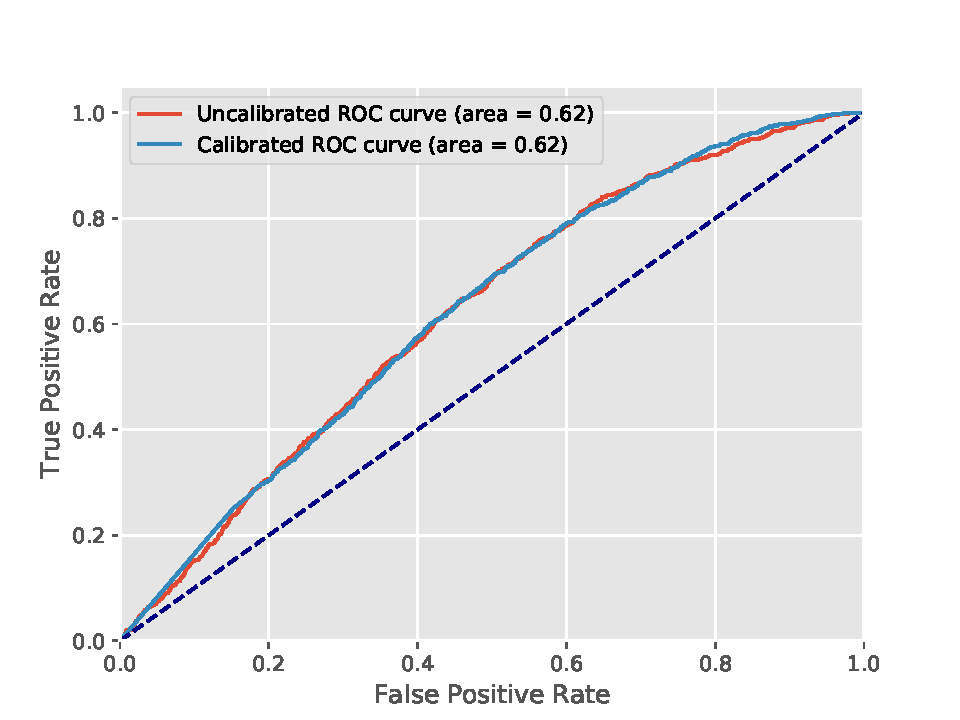
\includegraphics[width=0.6\textwidth]{figures/calibrationROC.pdf}
    \caption[Part 3: ROC curves showing the effect of calibration]{ROC curves showing the effect of calibrating the non-linear classifier.}
    \label{fig:calibroc}
\end{figure}

\subsection{Pricing Strategy}

Our pricing strategy was to identity and win contracts for the low risk customers. Our hypothesis was that by winning these customers' contracts we could minimize our claim-per-customer, and therefore could translate much of the revenue from selling contracts into profit. The price offered was the product of the frequency model (our calibrated base classifier) and the severity model (which was just the mean claim as written in the skeleton code) plus a margin. By setting a relatively high margin we were able to make good profits on the low risk customers and made us too expensive for the high risk customers so we did not win their contracts.

The successful execution of our strategy manifests through the performance of our insurance pricing agent. The mean price won was the lowest in the market (£44) (as we were aiming for the low-risk customers therefore had to offer cheap premiums to win them) and the mean loss incurred was also the lowest in the market at £35 (excluding agents that did not receive any claims). Additionally, our mean price offered was the highest in the market at £153. These imply all three of the pillars of our pricing strategy were successfully executed as we won the contracts of low risk customers, hence did not receive large claims and also did not win the contracts of high risk customers. This is how we managed to achieve a 3rd place ranking in the AI market.

\subsection{Linear Model Comparison}
\label{sec:linmodel}
Our linear model used a logisitic regression classifier (implemented as a one-layer neural network with sigmoid activation function utilising our existing code base (i.e. a single-layer perceptron)). Our linear model also performed well, making around half of the profit of our non-linear agent. 

The base classifier in the linear model performs similarly well to our non-linear base classifier. The PCA analysis in \autoref{section:explor} offers some insight as to why this is (as the part 2 data is a subset of part 3 data the results from running PCA on part 3 data do not differ significantly to the part 2 data). As noted in the earlier discussion of \atoref{fig:pca} in which we performed PCA the dataset, we have observed that the linear combinations of features account for the majority of correlation between labels and sets of features. As such, it is not surprising that the linear model performs relatively well. Indeed, we observed that many "semi-complex" network architectures actually performed worse than the single-layer perceptron, as their additional complexity was insufficient to capture any more nuanced and obscure trends in the data, whilst also hampering their ability to concisely represent the linear behaviour which predominantly determines the correlation in the data. 

To make matters worse, this means that we are faced with an optimization problem in which improving beyond the linear model requires a complicated network, which when coupled with the relatively small amount of data and dominance of the linear correlations makes it very difficult to converge on a superior optimum. This was indeed what we observed during the training and tuning of our final network architecture.

\newpage

\subsection{LabTS Complications}
We faced numerous substantial difficulties getting our implementations (for part 2 as well as part 3) to pass the LabTS tests. One such difficulty was converting categorical features to dummies so they could be used in the network. However, these ran into difficulties with LabTS and so (after spending a substantial amount of time identifying the issue) we decided to discard all categorical features. This harmed the performance of our model as it meant we discarded many useful features. This was one of the many complications we faced with LabTS, and cumulatively these took a substantial amount of time to overcome.

Our code never passed the tests on LabTS. However, it did pass the tests when we downloaded them and we gather from Piazza that this means our models should pass the tests upon assessment.



\bibliographystyle{IEEEtran}
\bibliography{refs}

% ==================================================== %
%% APPENDICES -----------------------------------------%
% ==================================================== %
\newpage
\begin{appendices}
\addtocontents{toc}{\protect\setcounter{tocdepth}{0}}
\section{Supplemental Figures}
\label{app:figures}
\addtocontents{toc}{\protect\setcounter{tocdepth}{1}}

\begin{figure}[h!]
    \ContinuedFloat*
    \centering
    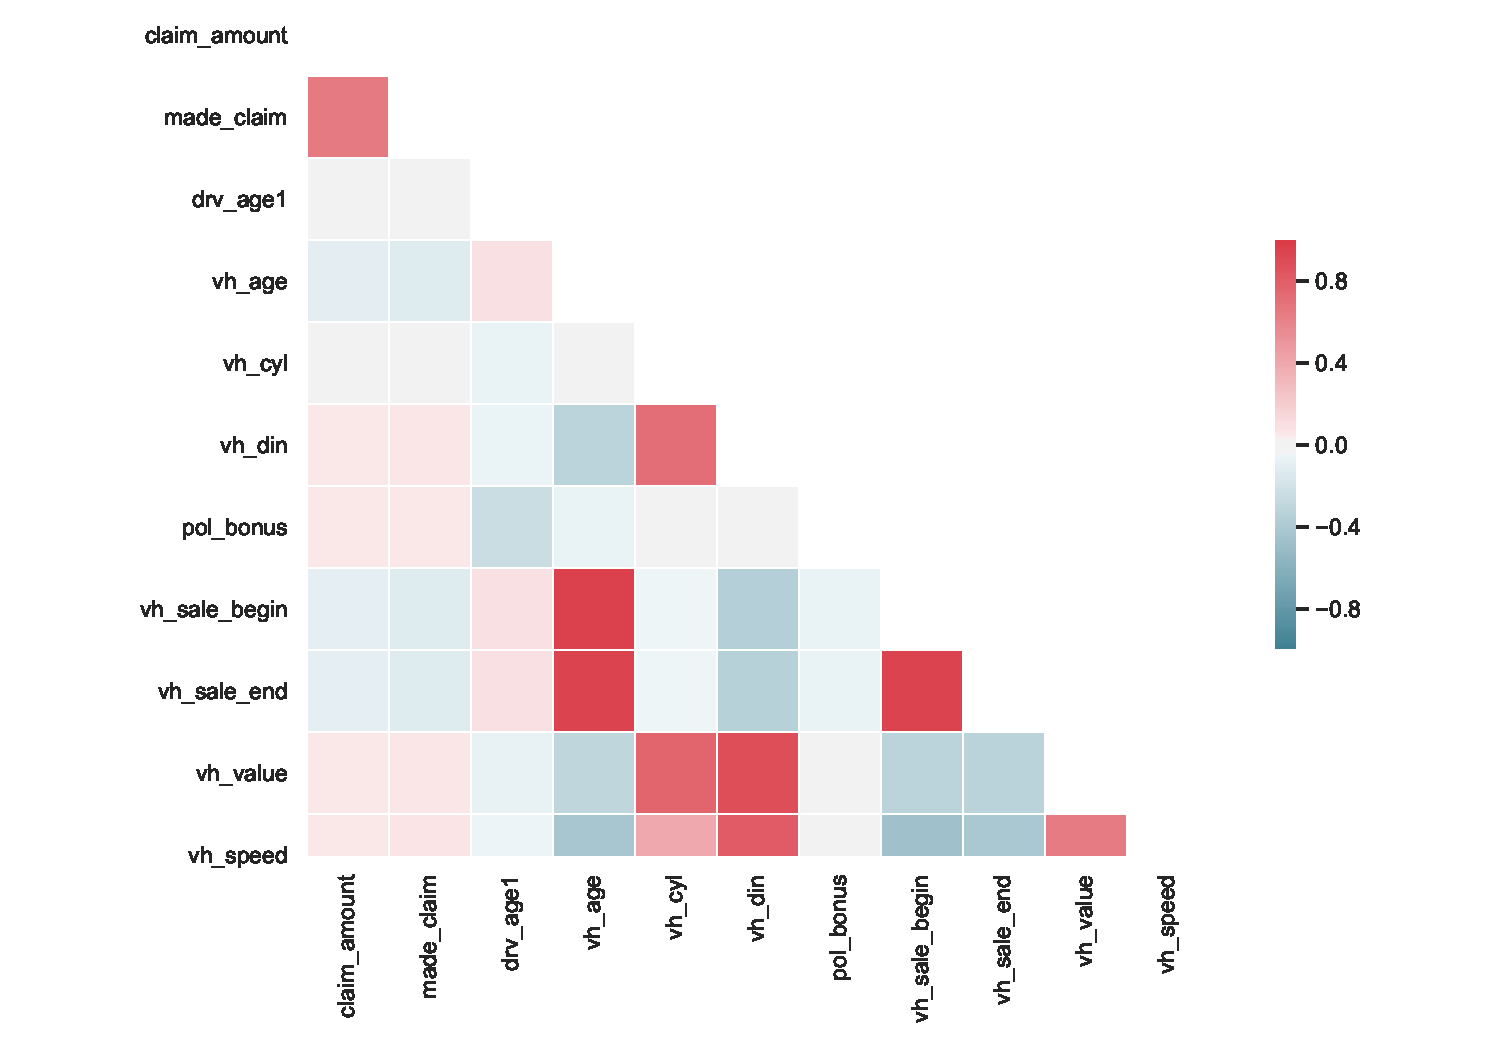
\includegraphics[width = 0.7\hsize]{./figures/corrplot.pdf}
    \caption[Correlation Matrix of Explanatory Variables]{Plot of the correlation matrix for \texttt{part2\_data.csv}. Dark red indicates a strong positive pairwise correlation between variables whereas dark blue indicates a strong negative correlation.}
    \label{fig:corrplot}
\end{figure}

\begin{figure}[h!]
    \ContinuedFloat*
    \centering
    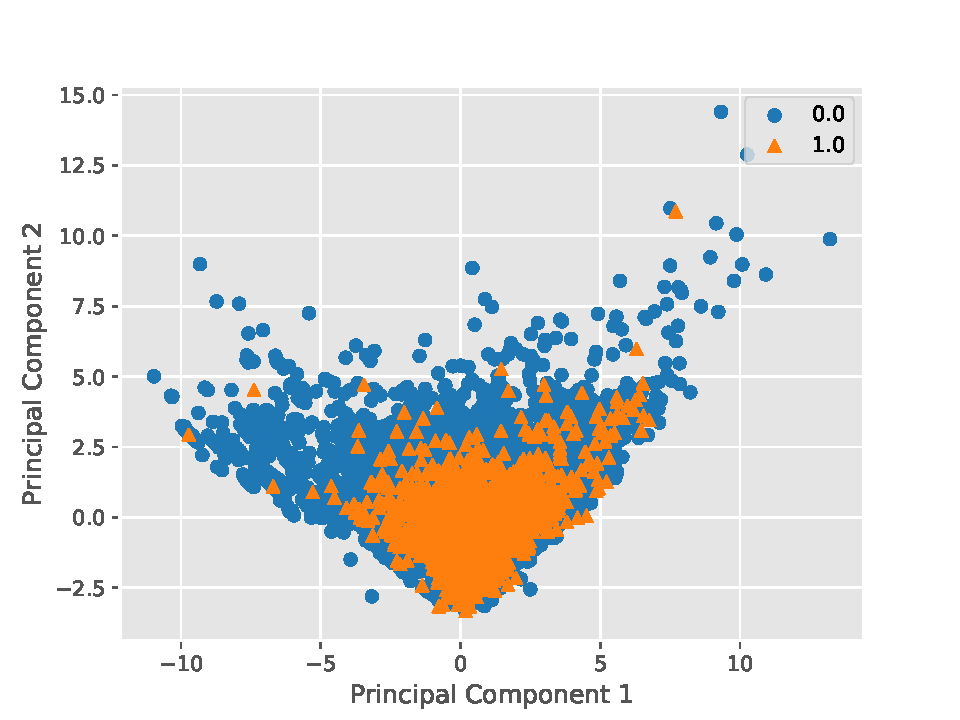
\includegraphics[width = 0.7\hsize]{./figures/pca.pdf}
    \caption[Scatter Plot of Explantory Variables post-Principal Component Analysis ($n=2$)]{Plot of \texttt{part2\_data.csv} post dimension reduction with Principal Component Analysis ($n=2$).}
    \label{fig:pca}
\end{figure}

\begin{figure}
\makebox[\linewidth][c]{%
\begin{subfigure}[b]{.6\textwidth}
    \centering
    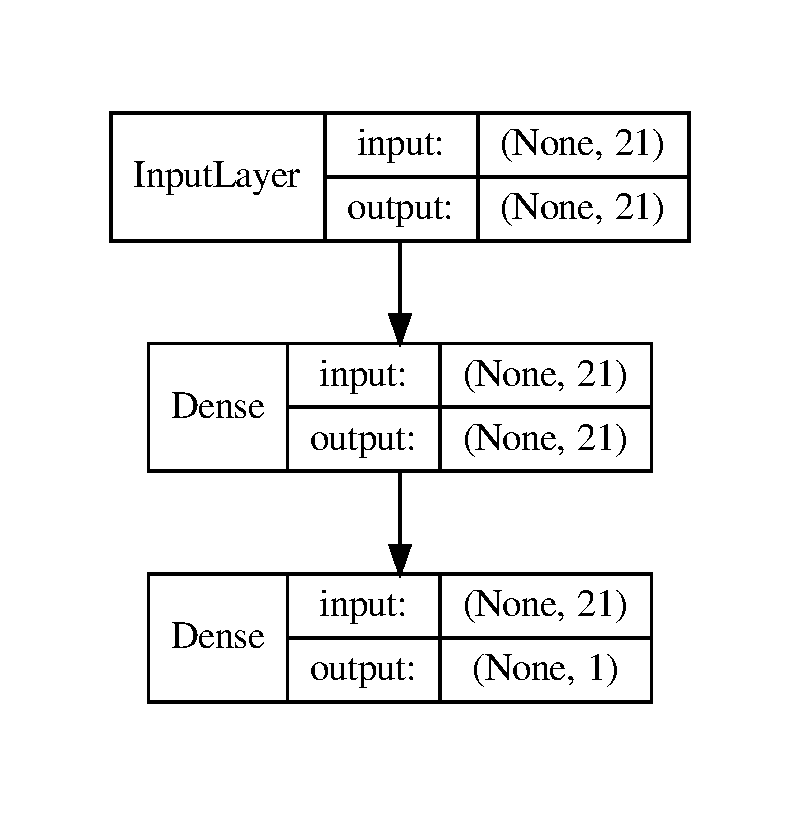
\includegraphics[width=0.8\textwidth]{figures/linear_model.pdf}
    \caption{Part 3 Linear model - Single Layer Perceptron}
    \label{fig:linmodel}
\end{subfigure}%
\begin{subfigure}[b]{.6\textwidth}
    \centering
    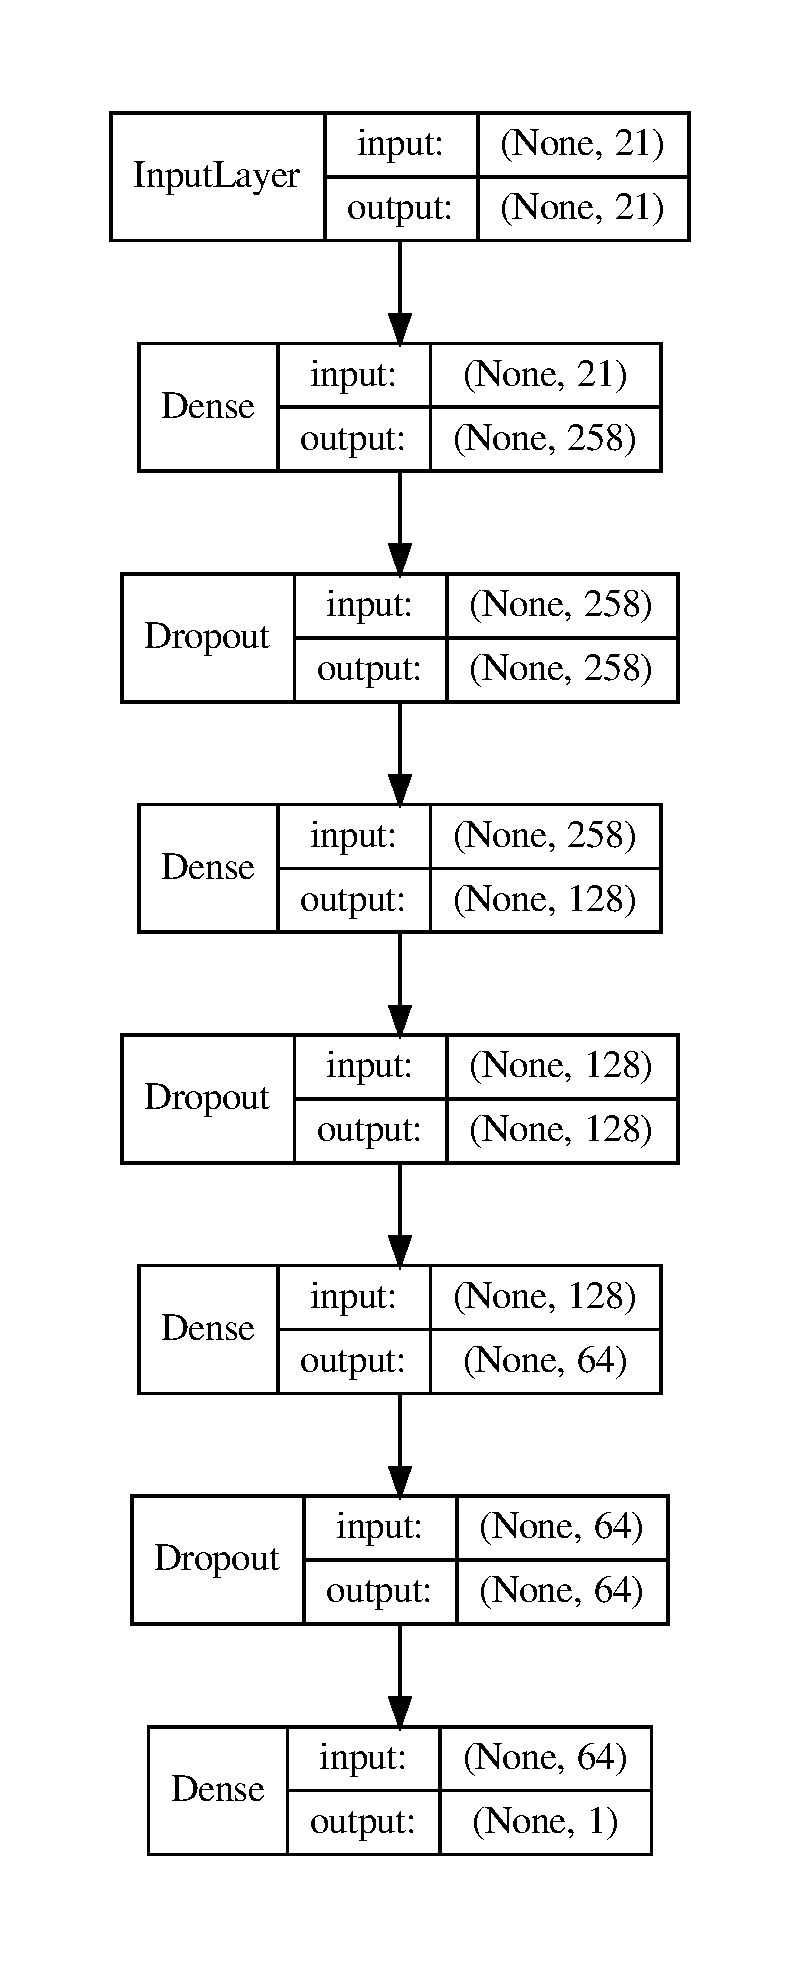
\includegraphics[width=0.8\textwidth]{figures/nonlinear_model.pdf}
    \caption{Part 3 Non Linear model.}
    \label{fig:nonlinmodel}
    \end{subfigure}%
}
\caption[Part 3 Linear and Non-linear Network Architectures]{Model Architectures}.
\label{fig:modelarchitectures}
\end{figure}
% \newpage
% \addtocontents{toc}{\protect\setcounter{tocdepth}{0}}
\section{Supplemental Results}
\label{app:results}
\addtocontents{toc}{\protect\setcounter{tocdepth}{1}}


% \newpage
% % \addtocontents{toc}{\protect\setcounter{tocdepth}{0}}
% \section{Code}
% \label{app:figures}
% \addtocontents{toc}{\protect\setcounter{tocdepth}{1}}

% \begin{lstlisting}[language=Python, caption=Python code]

% \end{lstlisting}
\end{appendices}

\end{document}

% \begin{algorithm}
% \footnotesize
% \SetAlgoLined
% \KwResult{Get feature \& value for splitting to deliver max entropy gain}
%  \For{feature in Features}{
%   sort data by feature\;
%   \For{unique value in feature}{
%   Split data into $subset_A, subset_B$ using this value\;
%     \For{$subset_A, subset_B$}{
%     Compute entropy for sub dataset (using \autoref{eq:entropy})\;
%     }
%   Compute entropy gain from splitting on feature (using \autoref{eq:entropy_gain})\;
%   Return value \& entropy gain for max entropy gain\;}
%   Return feature \& value for max entropy gain from splitting on each feature\;
%  }
% \caption{Determining splitting feature and feature value}\label{alg:splitting}
% \end{algorithm}

% \begin{table}[h!]
% \small\addtolength{\tabcolsep}{-5pt}
% \centering
% \begin{tabular}{|
% >{\columncolor[HTML]{EFEFEF}}l |l|l|}
% \hline
%               & \cellcolor[HTML]{EFEFEF}\textbf{Unpruned} & \cellcolor[HTML]{EFEFEF}\textbf{Pruned} \\ \hline
% \textbf{Clean} & 0.971                                     & 0.969                                  \\ \hline
% \textbf{Noisy} & 0.801                                     & 0.880                                   \\ \hline
% \end{tabular}
% \caption[Classification Rates for Datasets Before and After Pruning]{Classification rates for datasets before and after pruning}
% \label{tab:rates}
% \end{table}

% \begin{figure}
% \makebox[\linewidth][c]{%
% \begin{subfigure}[b]{.6\textwidth}
%     \centering
%     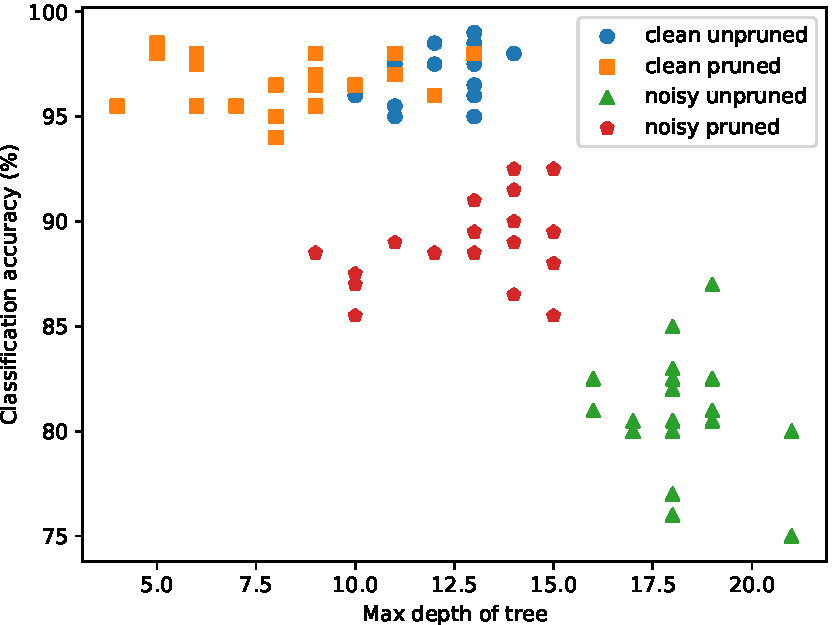
\includegraphics[width=0.8\textwidth]{figures/depth_plot.pdf}
%     \caption{Classification accuracy against the maximum depth of the trees.}
%     \label{fig:depth}
% \end{subfigure}%
% \begin{subfigure}[b]{.6\textwidth}
%     \centering
%     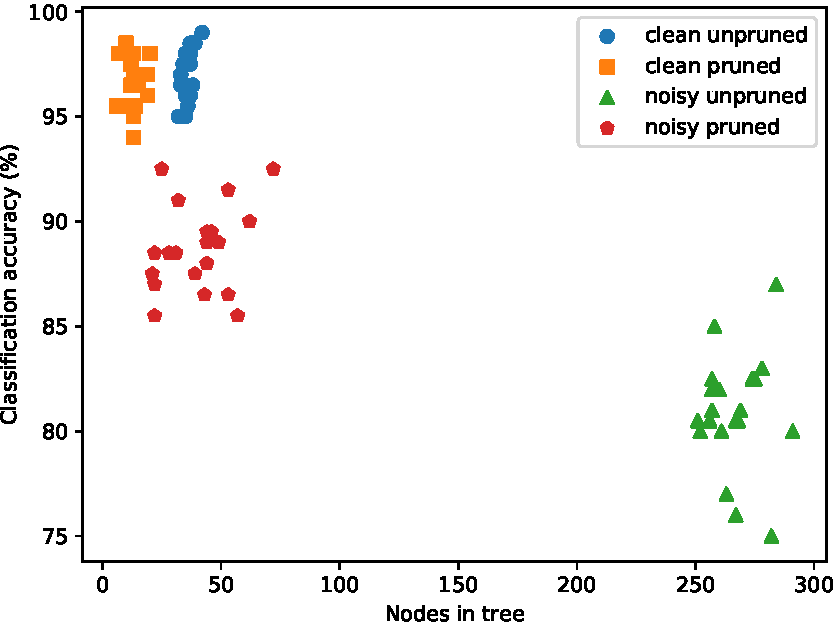
\includegraphics[width=0.8\textwidth]{figures/nodes_plot.pdf}
%     \caption{Classification accuracy against the number of nodes in the trees.}
%     \label{fig:nodes}
%     \end{subfigure}%
% }
% \caption[Effects of Pruning on Depth and Sparseness]{The effects of pruning on max tree depth and the number of nodes in the tree (both excluding leaves), and how these correlate with classification accuracy. In both plots, 20 trees were trained then tested before and after pruning.}
% \label{fig:pruning_effect_overview}
% \end{figure}


%%% Local Variables: 
%%% mode: latex
%%% TeX-master: t
%%% End: 














% \textcolor{red}{use an algoritm environment please}
% \\
% \begin{algorithm}
% \SetAlgoLined
% \KwResult{Write here the result }
%  initialization\;
%  \While{While condition}{
%   instructions\;
%   \eIf{condition}{
%   instructions1\;
%   instructions2\;
%   }{
%   instructions3\;
%   }
%  }
% \caption{How to write algorithms}
% \end{algorithm}




% \begin{itemize}
%     \item if the dataset has only one label, returns a leaf dictionary
%     \item else it finds optimal split, splits the dataset and runs the algorithm again on both parts of the dataset (left and right branches)
% \end{itemize}

% Finding the optimal split is the most complex part of the algorithm. The process of finding optimal split is described below:

% \begin{itemize}
%     \item First, the data is sorted based on the values of a single feature.
%     \item Second, the unique values of that feature are recorded.
%     \item Each of these unique values are used as split values, and the data is split into two based on whether the feature values are higher or lower than the split value.
%     \item For each of the resulting subsets, the entropy values are calculated using the formula 
    

    
%     \item For a given split value, the gain is calculated using the entropy values of its subsets (calculated in the last step). The gain is calculated using the formula:
    

    
%     \item This is repeated for each possible split value to find the split value that results in the highest gain. This is the optimal split value for the given feature.
%     \item All of the previous steps are repeated for each feature in the dataset, and the feature with the highest maximum gain is chosen as the best feature to split the dataset on. The split value that gives the maximum gain for this feature is used for the split. 
% \end{itemize}

% \begin{align}
%     Gain(S_{all}, S_{left},S_{right}) & =H(S_{all}) - Remainder(S_{left},S_{right}), \\
%     H(dataset) &= - \sum_{k=1}^{k=K}p_k*\log_2(p_k), \\
%     Remainder(S_{left}, S_{right}) &= \frac{|S_{left}|}{|S_{left}|+|S_{right}|}H(S_{left})+\frac{|S_{right}|}{|S_{left}|+|S_{right}|}H(S_{right})
% \end{align}